\documentclass[letterpaper,10pt,titlepage,draftclsnofoot,onecolumn,onesided] {IEEEtran}
\usepackage{listings}
\usepackage{underscore}
\usepackage[bookmarks=true]{hyperref}
\usepackage[utf8]{inputenc}
\usepackage[english]{babel}
%\usepackage{titling}
\usepackage{graphicx}
\usepackage{xcolor}
\usepackage[noadjust]{cite}
\usepackage{setspace}
\nocite{*}
\graphicspath{ {img/} }
%\usepackage{abstract}

\newcommand{\namesigdate}[2][4cm]{%
  \begin{tabular}{@{}p{#1}@{}}
    #2 \\[2\normalbaselineskip] \hrule \\[0pt]
    {\small \textit{Signature}} \\[2\normalbaselineskip] \hrule \\[0pt]
    {\small \textit{Date}}
  \end{tabular}
}
\newcommand{\studentnamesigdate}[2][4cm]{%
  \begin{tabular}{@{}p{#1}@{}}
    #2 \\[2\normalbaselineskip] \hrule \\[0pt]
    {\small \textit{Signature}} \\[2\normalbaselineskip] \hrule \\[0pt]
    {\small \textit{Signature}} \\[2\normalbaselineskip] \hrule \\[0pt]
    {\small \textit{Signature}} \\[2\normalbaselineskip] \hrule \\[0pt]
    {\small \textit{Signature}} \\[2\normalbaselineskip] \hrule \\[0pt]
    {\small \textit{Date}}
  \end{tabular}
}

\hypersetup{
    bookmarks=false,    % show bookmarks bar?
    pdftitle={Progress Report},    % title
    pdfauthor={Cramer Smith, Sam Lichlyter, Eric Winkler, Zach Schneider},                     % author
    pdfsubject={Progress Report},                        % subject of the document
    pdfkeywords={IFT, Report, Postal}, % list of keywords
    colorlinks=true,       % false: boxed links; true: colored links
    linkcolor=black,       % color of internal links
    citecolor=black,       % color of links to bibliography
    filecolor=black,        % color of file links
    urlcolor=blue,        % color of external links
    linktoc=page            % only page is linked
} 

\lstdefinestyle{customperl}{
  belowcaptionskip=1\baselineskip,
  breaklines=true,
  frame=L,
  xleftmargin=\parindent,
  language=Perl,
  columns=fullflexible,
  showstringspaces=false,
  basicstyle=\footnotesize\ttfamily,
  keywordstyle=\bfseries\color{green!40!black},
  commentstyle=\itshape\color{purple!40!black},
  identifierstyle=\color{blue},
  stringstyle=\color{orange},
  numbers=left
}
\lstset{escapechar=@, style=customperl}

% Document Title:
\def\doctitle{A Tool to Visualize the Structure of a Codebase Using Information Foraging Theory Design Patterns}
\def\doctype{Progress Report}
\def\doctype{Winter Midterm Update}
\def\team{Team Postal | Group \#38}

\markboth{Oregon State University}{\doctitle}

\begin{document}

\title{\Huge{\bfseries{\textsf{\doctitle}}}\\\textsf{\Large{\doctype}}\\\textsf{\large{\team}}}
\author{Cramer Smith, Sam Lichlyter, Eric Winkler, Zach Schneider}

\maketitle
\vfill

\setlength\parindent{0pt} \textbf{Abstract:} Developer tools are often complex pieces of software. 
Gathering and manipulating useful information for a programmer can often be a slow and costly process. 
By implementing Information Foraging Theory design patterns in the creation of these tools, the information collected may be more useful or produced faster. 
Information Foraging Theory is the theory and math behind the choices people make to maximize the value of the information they find versus the cost of getting that information.
The aim of this project is to develop a tool that will act as a proof of concept to this idea and increase developer efficiency.
Through the implementation of multiple IFT design patterns, the Postal team will create a developer tool that helps enforce and maintain code structure. 

\vfill

\pagebreak

\tableofcontents


\pagebreak

\section{Project Purpose and Goals}
Developer tools are often complex pieces of software. 
Gathering and manipulating useful information for a programmer can often be a slow and costly process. 
By implementing Information Foraging Theory design patterns in the creation of these tools, the information collected may be more useful or obtained faster. 
Information Foraging Theory (IFT) is the theory and math behind the choices people make to maximize the value of the information they find versus the cost of getting that information.
The aim of this project is to develop a tool that will act as a proof of concept for IFT and increase developer efficiency.

The Postal extension is being designed to allow developers to more quickly search through and better visualize their projects.
This extension will also help developers create clearer and cleaner code structure by offering reminders and suggestions about the best coding practices in the programming language they are currently using.
Any major errors or incompatibilities within the project or its files will be reported to the developer as well.

\section{Current Status}
	\subsection{Project Status}
	
	\subsection{Testing Status}

\section{Remaining Work}


\section{Problems and Solutions}
	\subsection{Fall Term}
	
	
	\subsection{Winter Term}
	
	
	\subsection{Spring Term}

\section{User Testing}
	\subsection{Testing Description}
	%Include our actual updated user questions, brief description of test projects, what we have users do
	
	\subsection{Measuring Results}
	%Include questionnaire questions and how we will measure effectiveness of project

\pagebreak	
\section{Images}
	\begin{figure}
		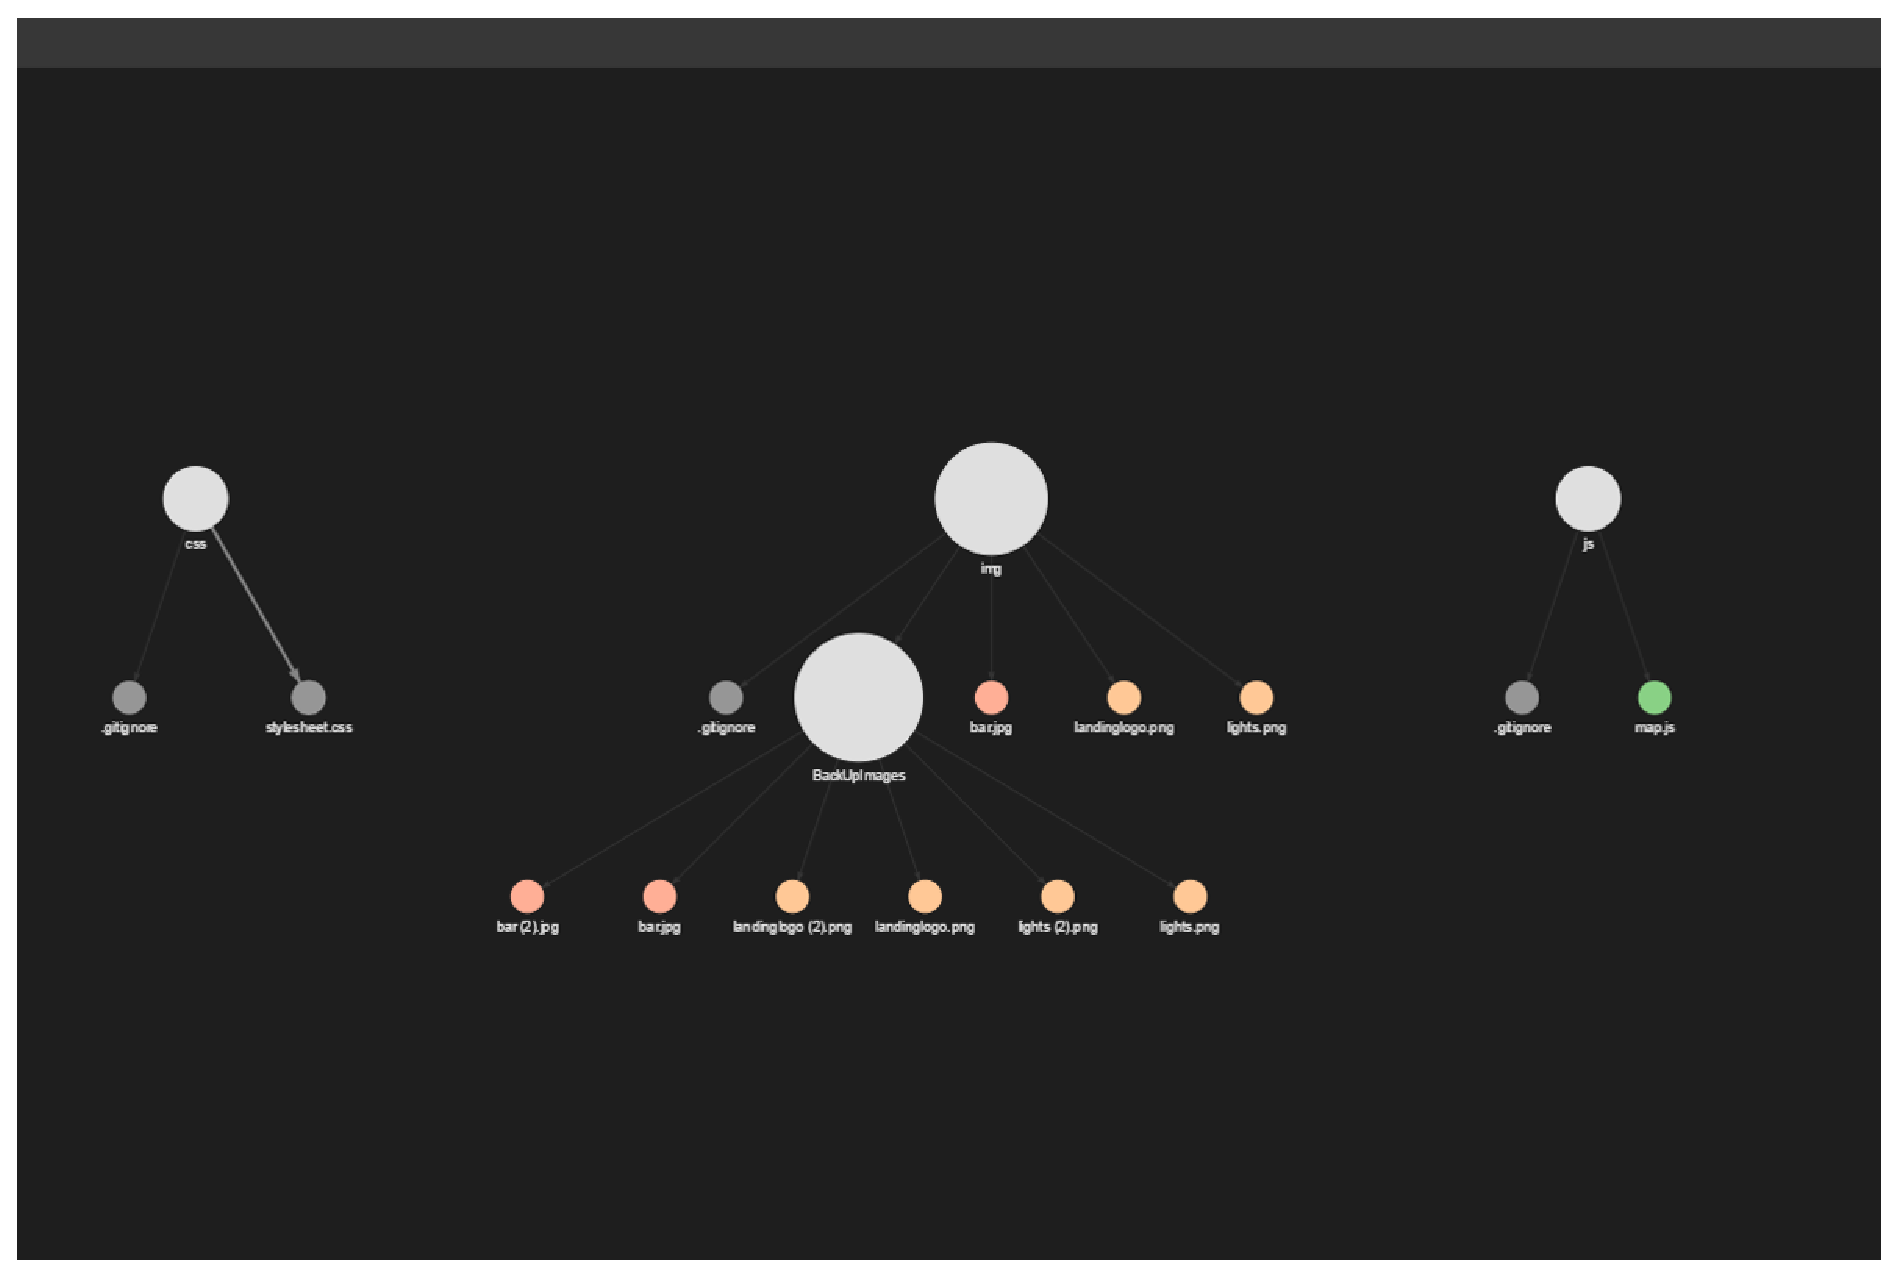
\includegraphics[width=400px]{capstoneUI1}
		\caption{Current User Interface}  %%UP TO DATE??????
	\end{figure}
	
	\begin{figure}
		\includegraphics[width=400px]{UpdatedDataStruct}
		\caption{Updated Data Structure}
	\end{figure}

\pagebreak
\section{Code Samples}
	\subsection{Example Grammar}
	This is the default grammar that parses HTML and PHP files for divs and links.
	
	\begin{lstlisting}
{
    "id" : 0,
    "title" : "html",
    "filetypes" : ["html", "php"],
    "rules" : [{
            "title": "div",
            "type": "tagged",
            "options" : {
                "tagStart": "<div",
                "namedOption" : "id=\"(.+?)\"",
                "tagEnd": ">",
                "closingTag": "</div>",
                "nodeColor": "blue"
            }
        }, {
            "title": "href link",
            "type" : "link",
            "options" : {
                "link": "href=[\"](.+?)[\"]",
                "nodeColor": "blue"
            }
        }, {
            "title": "includes link",
            "type": "link",
            "options": {
                "link": "include=[\"](.+?)[\"]",
                "nodeColor": "blue"
            }
        }, {
            "title": "body",
            "type": "tagged",
            "options" : {
                "tagStart": "<body",
                "tagEnd": ">",
                "closingTag": "</body>",
                "nodeColor": "blue"
            }
        }
    ]
}
	\end{lstlisting}

	\pagebreak
	\subsection{Recursive Get All Links}
	This function grabs all the links from the data structure of a specified file struct and it's children.
	\begin{lstlisting}
// Recursive function to get all links from this and children
function getAllLinksFromFileStructRecursive(FileStructID) {
    var links = [];

    // check parent
    if (DFS[FileStructID].links.length > 0) {
        for (var i = 0; i < DFS[FileStructID].links.length; i++) {
            var link = DFS[FileStructID].links[i];
            links.push(link);
        }
    }

    // check children
    if (DFS[FileStructID].subContainers.length > 0) {
        var childLinks = [];
        for (var i = 0; i < DFS[FileStructID].subContainers.length; i++) {
            var childFileStructID = DFS[DFS[FileStructID].subContainers[i].toFileStructid].id;
            childLinks = getAllLinksFromFileStructRecursive(childFileStructID);

            // push what we found to parents link list
            for (var j = 0; j < childLinks.length; j++) {
                links.push(childLinks[j]);
            }

        }
    } 

    return links;
}
	\end{lstlisting}

\pagebreak
\bibliographystyle{IEEEtran}
\bibliography{progress-report-team38}


\end{document}

